\documentclass[a4paper,11pt]{report}
\setcounter{secnumdepth}{3}
\usepackage{graphicx}
\usepackage{caption}
\usepackage[left=2cm,right=2cm]{geometry}
\usepackage{color}
% define the title
\author{Laboratoire de simulation du depistage}
\title{LSD Input GUI documentation}
\begin{document}
% generates the title
\maketitle
% insert the table of contents
\tableofcontents

\chapter{Introduction}
LSD's input GUI has been developed to create XML configuration files for SCHNAPS, LSD's simulator. The GUI displays the XML file in a way that allows non-programmers to easily interprete the data. It also contains multiple tools and buttons to modify the file. It is written in python, and uses the python bindings of the Qt library to display the graphics.

This document aims at presenting the functionalities of the GUI. It does not contain a deep explanation of the code underlying SCHNAPS nor the GUI itself. 

\chapter{SCHNAPS : A short introduction}
SCHNAPS is a generic simulator designed for health care modelling and simulations, parametrizable by configuration files and usable by non-programmers such as public health specialists. SCHNAPS stands for \emph{SynCHroNous Agent and Population-based Simulator}. Before starting to use the GUI, a small knowledge of how SCHNAPS behaves when running simulations is required. Mainly, two different steps occur during simulations.

\section{SCHNAPS : Generator}
At first, SCHNAPS generates virtual individuals. Each individual has its own variables. When supplying a configuration file to SCHNAPS, one has to ensure that these variables are correctly named, initialized, and that the information on how the variables are distributed in the virtual population is correct. Such subjects will be later discussed.

Individuals are generated at the start of a simulation. Also, the user can specify additional generations during the simulation.

\section{SCHNAPS : Simulator}
Once individuals have been generated, the simulator make sure every individual evolves during the simulation. Such evolution is done by ``routing" the individuals in trees that have been previously created by the user. Probabilities, either variables or fixed in the tree, affect the path taken by the virtual individuals. A path is often configured to modify variables, hence causing the so-called evolution.

\chapter{LSD input GUI}
The GUI itself is quite simple, consisting of a menu and multiple tabs. Basic tabs are always shown in the GUI while advanced tabs can be hidden/shown by the user.

%Population Tab section
\section{Population Tab}
The population tab is where you define the characteristics of the individuals that are going to be created during a simulation. In a SCHNAPS perspective, the virtual population is defined by demography variables and simulation variables, respectively named population variables and event variables in the GUI. Demography variables are variables that are predefined in files. Simulation variables are variables that are specific to a problematic/simulation. To make it simple, simulation variables live in a configuration file, while demography variables live beneath the GUI subsystem and are accessible in all configurations. The population tab is considered as a basic tab.

Moreover, it is possible for the user to specify multiple profiles. Each profile has its demography variables and its simulation variables.

%Main tab
\subsection{Main Tab}
Figure~\ref{fig:popTab} shows the different elements composing the population tab. One combobox, two tables and two submenu buttons are the principal elements of the tab. The \emph{Add} and \emph{Delete} buttons can be seen as part of the event variables table.
\begin{center}
\includegraphics[scale=0.4]{Pictures/Population/PopulationTab-Arrow.png}
\captionof{figure}{Population tab}
\label{fig:popTab}
\end{center}
\subsubsection{Profile ComboBox}
Choosing a profile refreshes the two tables with the population and event variables data associated with the selected profile. Ìnstructions on how to create a profile will be later discussed.
\subsubsection{Population variables table}
The population variables table lists information about the data found in the demography that is linked with the selected profile. Each line is a variable found in the file. As for the columns:
\begin{enumerate}
\item{Name : } Name of the variable, as found in the demography file
\item{Depends on : } Variable dependencies
\item{Range : } Variable possible values
\end{enumerate}
Note the checkbox located left of the name of the variables. The table lists all variables found in the demography. However, users might want to discard variables when generating the virtual population. Thus, only checked variables are kept.\footnote{When checking variables that have dependencies, ensure the dependencies are also checked. Otherwise, it will result in a simulator crash at runtime.} 
\subsubsection{Simulation variables table}
\label{subsubsec:simVarTab}
The event variables table lists information that the user has previously entered in the table. Figure~\ref{fig:simTable} shows the table and its buttons. Each line is a variable found in the configuration file for the currently selected profile. As for the columns: 
\begin{enumerate}
\item{Name : } Name of the variable, as found in the configuration file
\item{Type : } Variable type
\item{Depends on : } Variable dependencies
\item{Distribution : } Allows the user to edit variable's tree.
\end{enumerate}
\begin{center}
\includegraphics[scale=0.4]{Pictures/Population/SimVarTable.png}
\captionof{figure}{Event variables table}
\label{fig:simTable}
\end{center}

Unlike the population variables table, all columns of the event variables table can be edited, except for the \emph{Depends on} column. Double-click on the \emph{Name} column to edit variable's name.\footnote{If a variable name is edited and the edited variable is a dependency of another variable, ensure the modifications are also made in the dependent variable's tree. Otherwise, it will result in a simulator crash at runtime.}

Variable type is a more obscure concept that can be hard to understand by non-programers. Unfortunately, typing is essential for SCHNAPS. Double-click on the \emph{Type} column to edit variable's type.\footnote{Again, modifying a variable's type might cause problems if this variable is referenced somewhere in the trees. Be careful before doing so.} As seen in Figure~\ref{fig:typeComboBox}, a combobox will appear, allowing the user to choose between predefined types. More on types can be seen in Chapter~\ref{chap:treeEditor}.
\begin{center}
\includegraphics[scale=0.4]{Pictures/Population/typeComboBox.png}
\captionof{figure}{Type's edit combobox}
\label{fig:typeComboBox}
\end{center}

Double-clicking on the \emph{Distribution} column opens the tree editor. Here, the tree editor is used to set variable values, either in a fixed way or by statistical means. See Chapter~\ref{chap:treeEditor} for more details on the tree editor.

The \emph{Add} and \emph{Delete} buttons are used to add and delete variables from the event variables table. More on adding and deleting can be found in Section~\ref{subsec:TabAndList}.

%SubMenus
\subsection{Submenus}
Two submenus can be opened pressing the two submenu buttons seen in Figure~\ref{fig:popTab}.
\subsubsection{Profile manager submenu}
The \emph{Edit profile(s)} button opens the Profile Manager, as seen in Figure~\ref{fig:proMgr}. The \emph{Available profiles} list shows the currently defined profiles of the project.
\begin{center}
\includegraphics[scale=0.3]{Pictures/Population/Submenu/ProMgr.png}
\captionof{figure}{Profile manager}
\label{fig:proMgr}
\end{center}

\paragraph{Adding a profile}
Adding a profile can be achieved by pressing the \emph{Add from demography} button. When pressed, the Profile Adder is opened(see Figure~\ref{fig:proAdder}).
 
\begin{center}
\includegraphics[scale=0.3]{Pictures/Population/Submenu/ProAdder.png}
\captionof{figure}{Profile adder}
\label{fig:proAdder}
\end{center}

The line edit labeled \emph{Profile's name} is where you enter the name of your new profile. The \emph{Available demographies} list displays the demography files found in the Demography folder of the GUI application. For custom demography files to be listed as well, use the \emph{Add from file system} button to specify where other demographies rest in the file system. Once the demography has been chosen, you can add your new profile by pressing the \emph{OK} button. This will add a new profile, with empty event variables and an empty accept function. If you want one or both of the last two items to be copied from an existing profile, specify it using the appropriate combobox. More on the accept function can be found in section ~\ref{subsubsec:AccFunc}.

\paragraph{Removing a profile}
Pressing the \emph{Remove profile} button while a profile is selected in the \emph{Available profiles} list will delete the profile.

\paragraph{Cloning a profile}
To create a profile that is identical to a selected profile in the \emph{Available profiles} list(except for the name), use the \emph{Clone profile} button. As seen in Figure ~\ref{fig:clopro}, a combobox will appear, asking the user for the clone's name.

\begin{center}
\includegraphics[scale=0.3]{Pictures/Population/Submenu/ClonePro.png}
\captionof{figure}{Clone profile}
\label{fig:clopro}
\end{center}

\paragraph{Copy accept function}
It is possible to copy the accept function of the currently selected profile. Selecting the profile and pressing the \emph{Copy accept function} button will lead you to the Copy Wizard(see Figure~\ref{fig:copyWiz}). Just select the profiles you want the accept function copied to by checking the corresponding checkboxes.

\begin{center}
\includegraphics[scale=0.3]{Pictures/Population/Submenu/CopyWiz.png}
\captionof{figure}{Copy Wizard}
\label{fig:copyWiz}
\end{center}

\paragraph{Copy simulation variables}
It is possible to copy the accept simulation variables of the currently selected profile. Just use the same method as described above.

\subsubsection{Accept function submenu}
\label{subsubsec:AccFunc}
The accept function submenu is used to add restrictions on how the individuals are going to be generated. The simplest choice between the three radio buttons is the \emph{Accept all individuals} choice. This choice tells SCHNAPS to generate a population that is going to fit the distribution of the variables found in the demography file of the currently selected profile.

However, some simulations target specific groups of the population. For example, a simulation can target individuals that are in a 40 to 60 years old range. This is where the \emph{Simple accept function} choice can be useful. Figure~\ref{fig:accFunc} shows the Accept Function Manager. The above example is shown in the simple accept function area. User can choose between equals, greater or equal($>$=), smaller or equal($<$=) and between in the condition combobox. The second value line edit is disabled when the three first conditions are used(equals, $>$=, $<$=). The plus and minus signs are used to add or remove conditions on the same variable.\footnote{Conditions between variables can be seen as Logical AND. Conditions on the same variable can be seen as Logical OR}

To specify even more complex accept functions, you can use tree editor by selecting the \emph{Complex accept functions} radio button and pressing the \emph{Open tree editor} button.

\begin{center}
\includegraphics[scale=0.3]{Pictures/Population/Submenu/AccFunc.png}
\captionof{figure}{Accept function manager}
\label{fig:accFunc}
\end{center}

%Process Tab section
\section{Processes Tab}
\label{sec:procTab}
The processes tab is where you create all the subtrees that the are going to be used in a simulation. In medical terms, a model is often seen as one big tree with multiple branches. However, building such a tree using the tree editor would be complex, error-proned and quite difficult to understand. To make it simpler, processes can be seen as subtrees. It is the user's job to separate the theoretical model's tree in multiple logical subtrees. It takes a little bit of practice, but it is not so hard to achieve. 

%Main tab
\subsection{Main Tab}
Figure~\ref{fig:procTab} shows the different elements composing the processes tab.

\begin{center}
\includegraphics[scale=0.3]{Pictures/Processes/ProcessTab.png}
\captionof{figure}{Processes tab}
\label{fig:procTab}
\end{center}

\subsubsection{Processes List}
Processes of the currently loaded project are listed in the \emph{Processes list}. To modify a process name, double-click on the line. A line edit will appear, hence allowing the editing.\footnote{Ensure the modified process name is not referenced in other processes, or else this might lead to a simulator crash at runtime.} Use the \emph{Add} and \emph{Delete} buttons at the bottom of the list to add or remove processes. Use the {Open Tree Editor} button to edit the currently selected profile. More on the tree editor can be found in chapter~\ref{chap:treeEditor}

\subsubsection{Process Tree}
A preview of the currently selected process is shown in this area. The preview is in fact a picture that was taken using the tree editor. You can navigate through the preview using the scroll bars. However, editing is not possible.
%SubMenus
\subsection{Submenu}
Apart from the tree editor, only one submenu can be accessed using the Process tab. This menu can be opened by pressing the \emph{Load predefined process} button.
This submenu is intended for importing processes found in other project. Two projects simulating different problematics might have some of their processes similar enough to have one or more of them imported from one project to the other. When pressed, the user is asked to select a project where the processes to import can be found. The GUI then lists the processes of the selected project. Choice(s) can ben done checking the appropriate checkbox(es).

\begin{center}
\includegraphics[scale=0.3]{Pictures/Processes/ProcImport.png}
\captionof{figure}{Import submenu}
\label{fig:impProc}
\end{center}

%Parameters Tab section
\section{Parameters Tab}
\label{sec:paramTab}
When building trees using the tree editor, many nodes can be used to steer virtual individuals between different branches or to modify their variables. These nodes need information on how to interact with the individuals. A simple but common example would be a \emph{Treatment} node, where the price of the treatment has to be provided. Now, let's say this treatment can be found at 20 different locations in the model, all in different subtrees. And now, let's say you realize the price you entered initially was wrong. A lot of job ahead if you hardcoded the price.

This is one of the main reason why the parameters tab exists. Most of the nodes used in the processes offer two ways of entering the data ; by hardcoding it or by referring to it via a parameter. Using parameters is a good approach if :
\begin{enumerate}
\item{The same data is used at multiple places in the processes}
\item{The data is sensitive} 
\item{The data is going to be part of a sensitivity analysis} 
\end{enumerate}
%Main tab

\subsection{Main Tab}
As seen in Figure~\ref{fig:paramTab}, the main tab is quite simple. It consists of the \emph{Baseline parameters} table, which lists all the parameters of the currently loaded project. The \emph{Add} and \emph{Delete} buttons are used to add or remove parameters.

\begin{center}
\includegraphics[scale=0.3]{Pictures/Parameters/ParametersTab.png}
\captionof{figure}{Parameters tab}
\label{fig:paramTab}
\end{center}
Each line of the table describes a parameter. As for the columns:
\begin{enumerate}
\item{Name : } Name of the parameter, as found in the configuration file
\item{Type : } Parameter type
\item{Depends on : } Parameter value
\end{enumerate}
You can modify the listed parameters using the table. Double-click on the parameter's name to enable a line edit, allowing the edition of the parameter's name.\footnote{As always, changing a parameter's name when it is referenced in a process will lead to problems at runtime.}  Like variables, user has to specify parameter's type(See section~\ref{subsubsec:simVarTab}). Modifying the type can be achieved by double-clicking on the type of the currently selected parameter. Finally, to modify the value, double-click on the value of the currently selected parameter.
You can always delete parameters by using the \emph{Delete} button.

%Submenu
\subsection{Submenu}
Unlike most of the lists and tables found in the GUI, pressing the \emph{Add} button leads to a submenu, as seen in Figure~\ref{fig:paramAdd}. This submenu is used to create a new parameter.

\begin{center}
\includegraphics[scale=0.3]{Pictures/Parameters/AddParam.png}
\captionof{figure}{Parameters tab}
\label{fig:paramAdd}
\end{center}

First, name your parameter using the line edit. Then, select parameter's type using the combobox. Finally select if the parameter is a scalar(single value) or a vector, and enter the value in the line edit for a scalar parameter or using the list and the \emph{Add}/\emph{Delete} buttons if it is a vector. Vector parameters are used with branching nodes. See chapter~\ref{chap:treeEditor} for more details.

%Simulation Tab section
\section{Simulation Tab}
The simulation tab contains the metadata of the project.

%Main tab
\subsection{Main tab}
The simulation tab, as seen in Figure~\ref{fig:simTab}, is principally made of two tables named \emph{Scenarios list} and \emph{Population manager}. Some radio buttons, line edit and push button are also part of the tab, and this group of widgets is called the Clock Manager.

\begin{center}
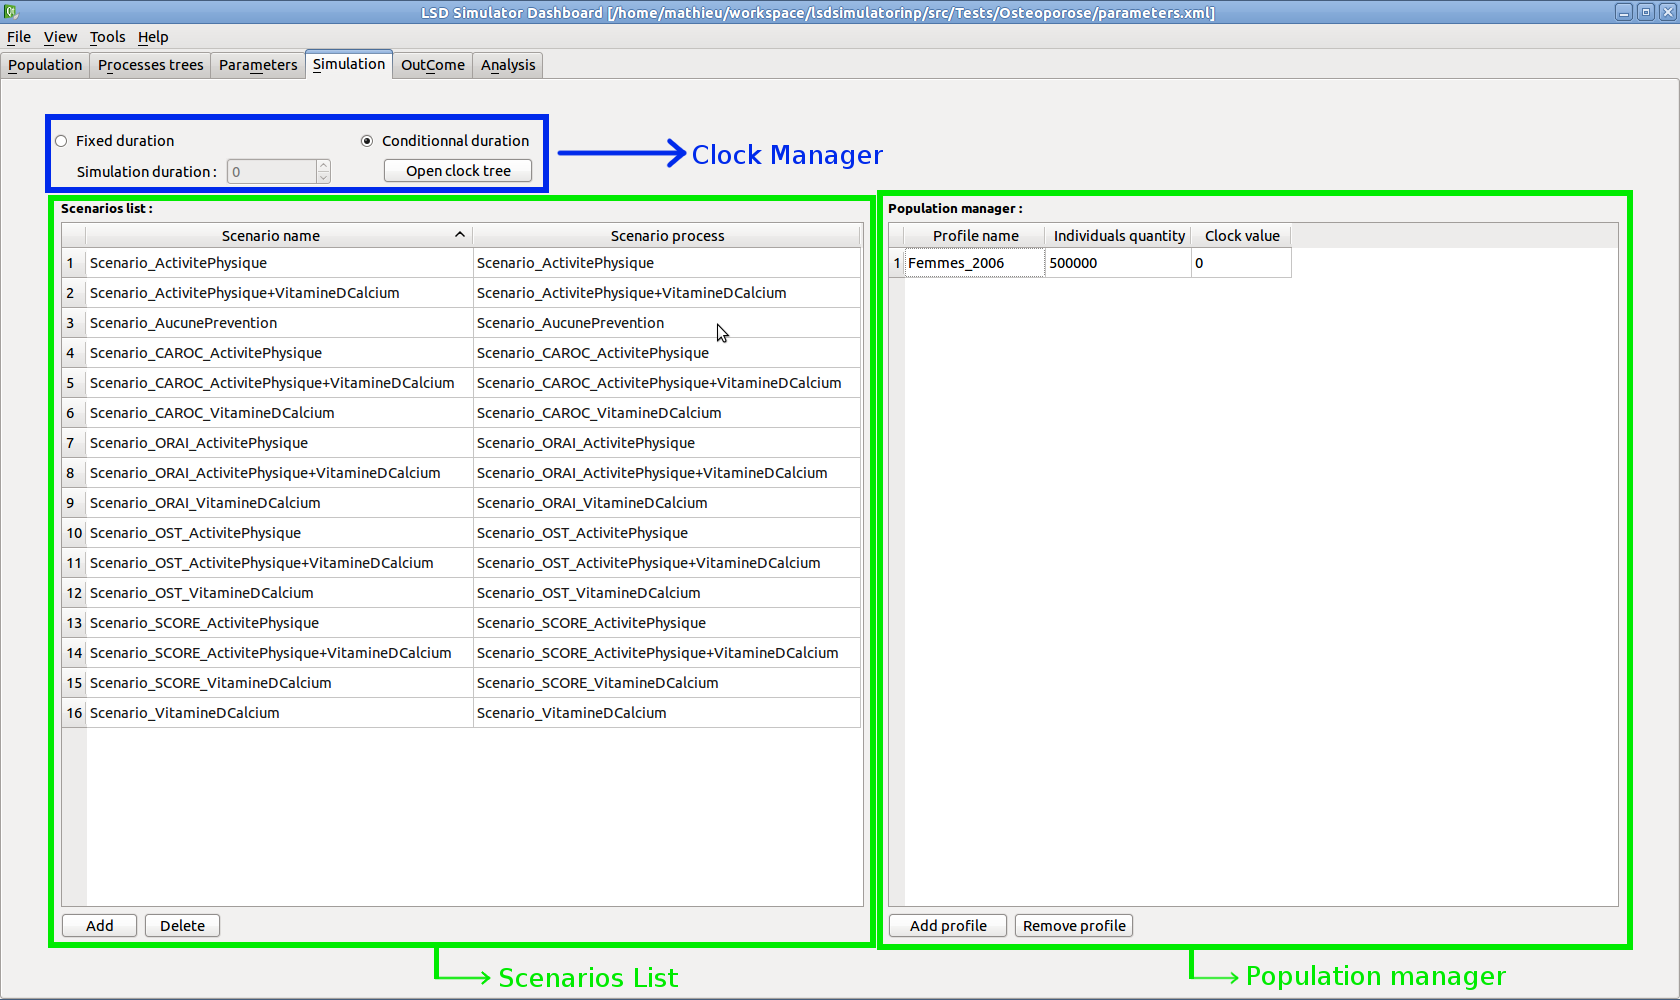
\includegraphics[scale=0.25]{Pictures/Simulation/SimulationTab-Arrow.png}
\captionof{figure}{Simulation tab}
\label{fig:simTab}
\end{center}

\subsubsection{Scenarios list}
\label{subsubsec:scenList}
A scenario is the first process SCHNAPS applies on all individuals when the simulation begins.\footnote{When individuals are introduced in the simulator during the simulation, the process is applied like if the simulation had just started for them.}. Each line in the \emph{Scenarios list} is a scenario. As for the columns :
\begin{enumerate}
\item{Scenario name : } Name of the scenario
\item{Scenario process : } Name of the associated process
\end{enumerate}
The scenario's associated process has to be created in the process tab(See section~\ref{sec:procTab}). Double-clicking on the cell will trigger a combobox, listing all processes found in the process tab. As for the name, it can be confusing. One good reason to make the scenario's name differ from the process name is that in complex projects with multiple scenarios, the name of the processes can become quite long. Naming the scenario with simple names(like numbers) can become handy. And since you only refer to scenarios when launching your simulation, you're not going to spend your time going through a lookup table searching for scenario 35's description, something that might happen if you don't use good naming conventions with your processes.

If this explanation doesn't satisfy your need for good reasons to justify the distinction between scenario's process and name, here's a better one. The GUI has two ``advanced'' tabs. One of them is the Environment tab(See section~\ref{sec:envTab}). The environment can be seen as a meta-individual, holding variables that are common to all virtual individuals. Like all other individuals , the Environment can go through a process that modifies its variables. So, a scenario can be a combination of two processes : one process that is applied to all the virtual individuals at the beginning of the simulation and one process that is applied to the environment, also at the beginning. In this case, naming a scenario takes all its sense. See section ~\ref{subsubsec:Pref} for details on how to enable this feature.

Using the \emph{Add} and \emph{Delete} buttons, you can add or remove scenarios to/from the project. Double-click on cells to modify their value. Scenario's name can be modified via a line edit while all processes found in the process tab(See section~\ref{sec:procTab}) are listed in a combobox.

\subsubsection{Population Manager list}
This is where you tell the simulator how to generate the individuals during the simulation. The columns of this table are :
\begin{enumerate}
\item{Profile name : } Name of the profile chosen for the generation
\item{Individual quantity : } Number of individuals to generate
\item{Clock Value : } Simulation step when the individuals are going to be created 
\end{enumerate}
Let \begin{math}x\end{math} be a value in Column 1, \begin{math}y\end{math} be a value in Column 2 and \begin{math}z\end{math} be a value in Column 3. So, for all lines, the simulator's generator creates \begin{math}x\end{math} individuals using profile \begin{math}y\end{math} and introduce them in the simulator at time \begin{math}z\end{math}. Use \emph{Add} and \emph{Delete} buttons to manage the generations. Modify the different cells by double-clicking on them. Quantity and time can be modified via a line edit while available profiles are listed in a combobox.

\subsubsection{Clock manager}
\label{subsubsec:clockMan}
There are two ways for the simulator to select the amount of steps the simulation is going to last. First one is to define a fixed number of steps using the \emph{Fixed duration} radio button. More complex possibilities can be set using the \emph{Complex duration} radio button, and pressing the \emph{Open clock tree} button. A complex condition ends the simulation when clock's tree returns True(see chapter~\ref{chap:treeEditor}).

%Outcome Tab section
\section{OutCome Tab}
In most cases, half of individual variables found in a simulation are control or state variables. Usually the user care more or less about such variables final values. The outcome tab is there to tell the simulator which variables to keep and write to a file and which one to throw away at the end of a simulation.

\begin{center}
\includegraphics[scale=0.3]{Pictures/Outcome/OutcomeTab.png}
\captionof{figure}{Outcome tab}
\label{fig:outTab}
\end{center}

\subsection{Profile List}
The \emph{Available profiles} list displays the profile found in the population tab. When clicking on a profile, it updates the \emph{Available variables} list.

\subsection{Variable List}  
\label{subsec:outVar}
The \emph{Available variables} list displays the variables found in the currently selected profile. It first lists the population variables in alphabetical order. The event variables are then listed, also in alphabetical order. There's a checkbox next to each variable name, that can be checked or unchecked, depending if the user wants to keep the variable or not. Population variables that are not chosen in the population tab at first are going to be listed, but the user won't be able to interact with their checkbox.

\subsection{Environment List}
When the environment is used in a simulation, environment variables are also listed. Rad the section above for more details.

%Analysis Tab section
\section{Analysis Tab}
\label{sec:advTab}
The analysis tab is still under construction and might be modified/renamed or even disappear.

%Advanced Tab function
\section{Advanced Tabs}
Advanced tabs are tabs that are not initially shown in the tab list. When enabled\footnote{See section~\ref{subsec:View} for more details on how to enable advanced tabs.}, they allow the user to define complex elements of the simulation. Unlike normal tabs, they do not need to be filled.

\subsection{Environment Tab}
\label{sec:envTab}
The environment, is some kind of master individual holding variables that are common to all virtual individuals. The environment is often used to carry control variables. A simple but telling example would be simulations where all individuals have to be ``dead'' for the simulations to stop. The common way to proceed in such cases is to keep a variable in the environment that registers the total number of individuals at the beginning of the simulation. This number is decremented when a virtual individual ``dies''. Once it has reached zero, the simulation is over. This is done by defining a complex duration for the clock(see section~\ref{subsubsec:clockMan}).

The environment tab is quite simple. It consists of the \emph{Environment variables} table and the \emph{Add/Delete} buttons. Each line of the table is a variable. The three colums are respectively the variable's name, type and value. Each cell can be double-clicked so the value it contains can be modified\footnote{As always, make sure you know what you're doing before changing a variable's name or value}. Like all other tables of the GUI, lines can be added or removed using the \emph{Add/Delete} buttons.

Finally, when shown, the environment tab is the first tab of the GUI.

\begin{center}
\includegraphics[scale=0.3]{Pictures/Environment/EnvironmentTab.png}
\captionof{figure}{Environment tab}
\label{fig:envTab}
\end{center}

\subsection{Observers Tab}
The observers tab is probably the most difficult tab to understand. Even though, it can be very useful in most projects. 

Take a simulation where each clock steps represents a normal year in a virtual individual's life. Each time the clock's value changes, some individual variables have to be updated(age, death probability,etc...). The user will usually do this by creating a process that modifies the variables. He then will list in the observers tab all the processes that have to be applied to individuals when the clock's value changes.

Even though the observers tab is considered as advanced, its layout remains simple. It consists of the \emph{Clock observers} table and the \emph{Add/Delete} buttons. Each line represents an observer. The first column is the name of the observer's process. As for the \emph{Targets} column, it dictates to who the process is going to be applied :
\begin{enumerate}
\item{individuals : }Apply the observing process to all virtual individuals
\item{environment : }Apply the observing process to the environment
\item{current individual : }Deprecated. Might be deleted in a near future. 
\end{enumerate}
The observing process and the targets can both be modified by double-clicking on the cell. Note that:
\begin{enumerate}
\item{The observers are executed before any other processes at the beginning of a clock step.}
\item{The observers are executed sequentially in order they appear in the table.}
\end{enumerate}
The last statement is quite important. If observing processes results depend on variables that are modified in other observers, make sure the sorting of your observers is correct. For example, if a process updating the death probability of the individuals depends on Age(also modified in an other observer), make sure the observer modifying the age is placed before the observer updating the death probability in the table.

Finally, when shown, the observers tab is located between the processes and the parameters tab.

\begin{center}
\includegraphics[scale=0.3]{Pictures/Observers/ObserversTab.png}
\captionof{figure}{Observers tab}
\label{fig:obsTab}
\end{center}

%Menu section
\section{Menus}
%File menu
\subsection{File}
The file menu holds different command for managing the project files and leaving the application.

\subsubsection{Open}
The \emph{Open} command pops open a file system navigator(see Figure~\ref{fig:fSysNav}) so you can select a project to open. LSD input GUI projects wear a \textbf{.lsd} file extension. Open command can be triggered using the \emph{Ctrl-O} shortcut.

\begin{center}
\includegraphics[scale=0.3]{Pictures/Menu/FileSysNav.png}
\captionof{figure}{File system navigator(Linux)}
\label{fig:fSysNav}
\end{center}

\subsubsection{Start New Project}
The command's name says it all. It starts a new empty project.

\subsubsection{Save}
\label{sec:save}
Saves the current project. \emph{Save} command can be triggered using the \emph{Ctrl-S} shortcut.

\subsubsection{Save As}
Opens a file system navigator and asks the user to give a new name to the currently loaded project so it can be saved as a new project. \emph{Save As} command can be triggered using the \emph{Ctrl-Shift-S} shortcut.

\subsubsection{Open plugin}
\label{sec:pluginmgr}
The \emph{Open Plugin} command is used to add functionalities to the GUI. These functionalities are, for the moment, only related to the tree editor. \emph{Open Plugin} command can be triggered using the \emph{Ctrl-Shift-O} shortcut.

Once activated, the command opens the Plugin Manager, as seen in Figure~\ref{fig:pluginMgr}. The plugin manager lists the different plugins used by the currenty loaded project. It also lists currently unused plugins that are found in the GUI folders. If a plugin is located somewhere else on the file system, it can be added using the \emph{Browse} button. Select plugins in one of the two lists and use the arrows to add or remove plugins from the currently selected project. More on plugins can be found in section~\ref{sec:plugins}.

\begin{center}
\includegraphics[scale=0.3]{Pictures/Menu/PluginMgr.png}
\captionof{figure}{Plugin manager}
\label{fig:pluginMgr}
\end{center}

\subsubsection{Exit}
Leaves the application. \emph{Exit} command can be triggered using the \emph{Ctrl-Q} shortcut.

%View menu
\subsection{View}
\label{subsec:View}
The view menu allows the user to show/hide the advanced tabs(see section~\ref{sec:advTab}) via checkboxes.

%Tool menu
\subsection{Tools}
The tools menu holds various extra functionalities of the GUI.

\subsubsection{Take Screenshot}
Takes a screenshot of what is currently visible in the GUI's main Window.\emph{Take Screenshot} command can be triggered using the \emph{Ctrl-T} shortcut. Once the screenshot has been taken, user is asked to save the picture somewhere on the file system. Actually, pictures can only be saved in a .png format. More types may be implemented in the future.

\subsubsection{Check variables validity}
For all simulation variables of all profiles, this command checks if there are any errors located in the tree. More on validation can be read in section~\ref{sec:validator}.

\subsubsection{Check processes validity}
For all processes, this command checks if there are any errors located in the tree. More on validation can be read in section~\ref{sec:validator}.

\subsubsection{Check all}
\label{subsubsec:check}
Runs the command of the two previous section sequentially.

\subsubsection{Demography editor}
Demography files can be added or edited via the demography editor. When pressed, the demography editor starts by asking the user if he wants to create a new demography or to load an existing one. The demography editor is then opened. Figure ~\ref{fig:demoEditor} shows the demography editor where an existing demography has been loaded.

\begin{center}
\includegraphics[scale=0.3]{Pictures/Menu/DemoEditor.png}
\captionof{figure}{Demography editor}
\label{fig:demoEditor}
\end{center}

The demography editor shows the name fo the file currently being edited. Each line of the table corresponds to a variable found in the file. As for the columns: 
\begin{enumerate}
\item{Name : } Name of the variable, as found in the demography file
\item{Type : } Variable type
\item{Depends on : } Variable dependencies
\item{Range : } Variable possible values
\item{Distribution : } Allows the user to edit variable's tree.
\end{enumerate}

As always, double-click on a cell to edit value. Note that \emph{Depends on} and \emph{Range} cells are not editable. Use the \emph{Add/Delete} buttons to add or remove variables to/from the demography.

You can also change the currently edited demography by pressing the \emph{Load Demography} button. A file system navigator will then open, asking you to select a demography file to edit.

Finally, note that modifications brought to the demography won't be effective until you save them. Saving is offered when the user presses the \emph{Ok} button or presses the \emph{Load Demography} button.
 Pressing the \emph{Cancel} or the Close button exits the demography editor without saving changes.

\subsubsection{Configuration file generator}
SCHNAPS uses pseudo-random number generation for its Generator and its Simulator. SCHNAPS Simulator and SCHNAPS Generator use pseudo-random generators, which can be configured via the configuration file generator. That makes a lot of generators :
\begin{enumerate}
\item{SCHNAPS Generator : } Part of SCHNAPS in charge of creating the virtual individuals
\item{Pseudo-random generator : } Piece of software in charge of creating numbers in a pseudo-aleatory manner
\item{Configuration File generator : } See Figure~\ref{fig:confGen}
\end{enumerate}
A pseudo-random generator uniformly generates numbers. However, it needs a number, called a seed, to start working properly. The reason why it is called a \textbf{pseudo-random} generator is that given the same seed when it is initialized, it will always generate the same exact sequence of numbers. Given this information, we can infer that, for two identical configuration files(except for the seeds):

\begin{center}
  \begin{tabular}{ |c | c | c | }
    \cline{2-3}
    \multicolumn{1}{c|}{} & Same simulator seeds & Different simulator seeds \\ \hline
    Same generator seeds & Same population & Same population \\ & Same events & Different events  \\ & Same output & Different output \\ \hline
    Different generator seeds & Different populations & Different populations \\ & ? & Different events  \\ & Different output & Different output \\
    \hline
  \end{tabular}
\end{center}

Note the question mark. Given a model where the paths are never influenced by individual variables, we can argue that for this combination of seeds, the same events will happen for different individuals. Most likely, this will never be the case. We can almost always replace the question mark by a \emph{Different events}. 

So, since we are not interested in simulating the same exact thing forever, let's take a look at the different options. First, the user is asked to select which of the Simulation, Generation or both seeds he wants to generate. Depending on the system's hardware and/or operating system, seeds can take 32 bits or 64 bits values. The user has to be aware of this and choose the right bit's length(choosing 32 bits on a 64 bits system is not a big deal but the opposite may certainly lead to problems). Finally, user has to choose how many files he want to create. The files are going to be created inside the project's directory. Pressing the \emph{Ok} button generates the files.

\begin{center}
\includegraphics[scale=0.3]{Pictures/Menu/FileGen.png}
\captionof{figure}{Configuration file generator}
\label{fig:confGen}
\end{center}

%Help menu
\subsection{Help}
For the moment, this section doesn't really contain any help or support doc. This is going to be done in a near future.

\subsubsection{About}
The \emph{about} command displays information about the GUI. It also lists what version of Python, Qt and PyQt is installed on the computer, as well as the name of the operating system.

\begin{center}
\includegraphics[scale=0.3]{Pictures/Menu/About.png}
\captionof{figure}{About}
\label{fig:About}
\end{center}

\subsubsection{Preferences}
\label{subsubsec:Pref}
To display the preferences of the application, use this command. \emph{Preferences windows} is going to be extended in the future. For now it contains three checkable/uncheckable options:
\begin{enumerate}
\item{Automatically load wizard at startup :} Loads wizard at startup.(See section~\ref{chap:wizard})
\item{Automatically check model at startup :} Checks the project for errors at startup.(See section~\ref{subsubsec:check})
\item{Show environment target in scenario model/view : } Adds a column to the scenarios list.(See section~\ref{subsubsec:scenList}) 
\end{enumerate}
\begin{center}
\includegraphics[scale=0.3]{Pictures/Menu/Preferences.png}
\captionof{figure}{Preferences}
\label{fig:preferences}
\end{center}

%Control section
\section{Control}
\subsection{Tables and Lists}
\label{subsec:TabAndList}
\subsubsection{Adding and Deleting}
Tables and lists that support the addition and deletion have the following behavior:
\begin{enumerate}
\item{Selecting a line in the table before pressing the \emph{Add} button inserts a new item under the selected item}
\item{If no selection is made, item is inserted at the end of the table} 
\item{As for deletion, at least one item has to be selected for the deletion to proceed} 
\item{It is possible to select more than one item for multiple deletion} 
\end{enumerate}

\subsubsection{Sorting}
Most tables and lists support sorting of the displayed items.
\begin{enumerate}
\item{Pressing the title of the columns sorts the table in Ascending/Descending order}
\item{Drag and drop is enabled so custom sorting can be achieved}
\end{enumerate}
When saving or opening a project, the GUI makes sure the items are ordered the way they were when the user last modified the configuration file. 

\subsubsection{Colors}
Colors might appear in tables where the tree editor can be launched. In fact, the words contained in the cells of the first column will have different colors. They are meant to be a quick display of the status/validity of the tree. Colors mean :

\begin{center}
\begin{tabular}{|c c|}
\hline
\textcolor{black}{Black} & Tree validity is unknown \\
\textcolor{green}{Green} & Tree is error/warning free\\
\textcolor{red}{Red}& Tree has errors\\
\textcolor{yellow}{Yellow}& Tree has warnings\\
\hline
\end{tabular}
\end{center}

Tree validity is unknown when the tree validator has not yet been able to validate the tree.(See section~\ref{sec:validator}) 

%Tree editor
\chapter{LSD tree editor}
\label{chap:treeEditor}
The LSD tree editor can be seen as a whole different application. LSD's tree editor displays the information located in xml files in a user-friendly way. It has been developed to help non-programmers to read and write XML files. No deep knowledge of the xml architecture is required. In fact, most users will end up using the tree editor without even knowing what kind of file lays behind.

\section{Layout}
First, let's have a look at the tree editor and its components.
\begin{center}
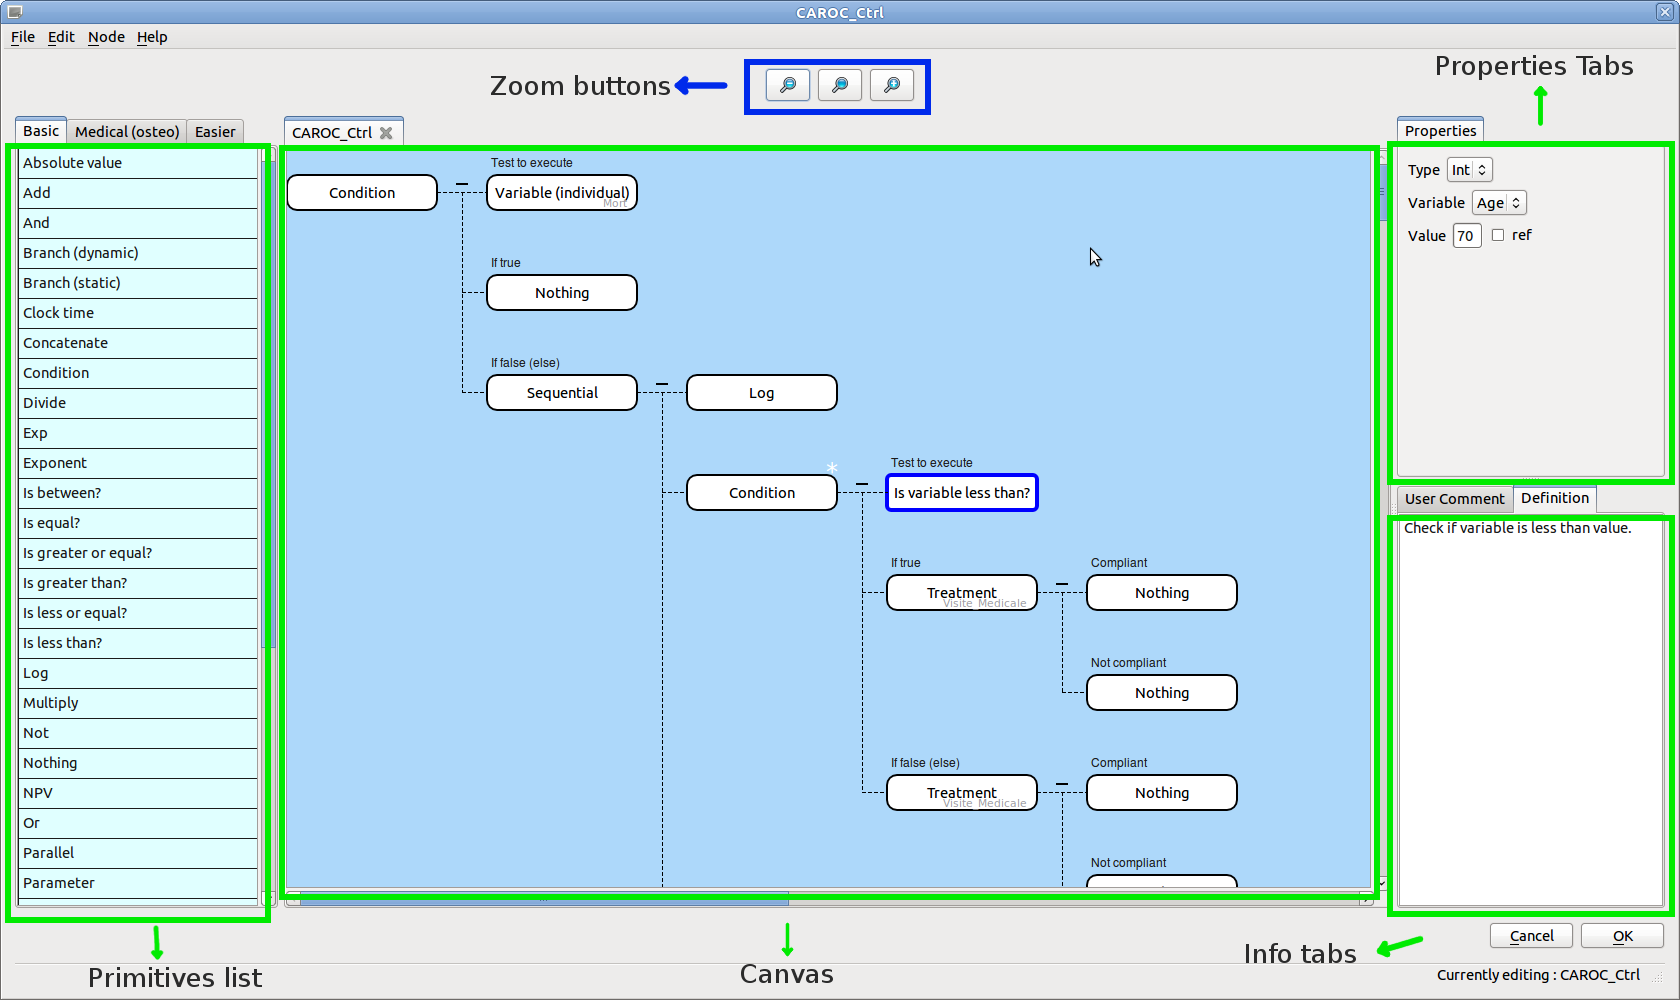
\includegraphics[scale=0.25]{Pictures/TreeEditor/TreeEditor-Arrow.png}
\captionof{figure}{Tree Editor}
\label{fig:treeEditor}
\end{center}

There are 4 principal components in the tree editor:
\begin{enumerate}
\item{Canvas} : Graphical representation of the XML tree
\item{Primitives list} : Lists the available primitives of the currently loaded plugins  
\item{Properties Tab} :  Lists currently selected item's attributes
\item{Info tabs} : Lists currently selected item's additional information
\end{enumerate}

%Canvas
\subsection{Canvas}
The canvas is where a graphical, user-friendly representation of the XML tree is drawn on a blue background.

\paragraph{Rounded corner rectangle}
Each rectangle represents a node in the xml tree. The name of the node is located in the center of the rectangle, and is often a good indicator of its function in the tree. A node can have 0, 1 or multiple children. A node normally has a parent, unless it is the root of the tree. Nodes will often be called primitives in the present chapter, as they can take a limited set of values defined in the primitives list. When the borders of a rectangle are drawn in blue, it means the node is the currently selected itme of the tree. The borders can also be painted in red or in yellow. See section~\ref{sec:validator} for more details.

\begin{center}
\includegraphics[scale=0.4]{Pictures/TreeEditor/nodeSelected.png}
\captionof{figure}{A selected node}
\end{center}

\paragraph{+ or - signs}
The plus/minus signs are used to expand/collapse parts of a tree. Simply click on the sign to expand/collapse a subtree. Plus sign's color indicates the validity state of its subtree. See section~\ref{sec:validator} for more details.

\paragraph{Dashed lines}
Dashed lines are drawn to link a child to its parent. 

\paragraph{Asterisks}
Users can write comments for each nodes of the tree. Normally, user will only write comments for nodes they judge complicated to understand, or for critical parts of the tree. When a node has been commented, a white asterisk is drawn over its rectangle. To see the comment, click on the node and the comment will be displayed in the comment window of the info tabs(see section~\ref{sec:infoTab}).
 
\begin{center}
\includegraphics[scale=0.4]{Pictures/TreeEditor/nodeAsterisk.png}
\captionof{figure}{A commented node}
\end{center}

\paragraph{Node tag}
Node tags are small pieces of text located over the nodes. They are hints to help the user understand what kind of node the parent expects to have at the position the node tag is located. In figure~\ref{fig:nodeTag}, node tags are labeled \emph{Compliant} and \emph{Not compliant}. Hence, first branch is what happens when patient is compliant to the treatment and second branch is what happens when patient is not compliant.
 
\begin{center}
\includegraphics[scale=0.4]{Pictures/TreeEditor/nodeTag.png}
\captionof{figure}{Node tags}
\label{fig:nodeTag}
\end{center}

\paragraph{Branch tag}
Branch tags are small pieces of text drawn to the left of branches. When a node branches a virtual individual in one of multiple choices, branch tags indicate which choice is associated with which branch. Choices can either be probabilities or possible variable values. Double-click on the branch tag to edit the value. Note that if the choice is a reference to a parameter, it cannot be edited\footnote{See section~\ref{sec:propTab} for more details on references.}. When a red exclamation mark is shown, it means a value hasn't been yet entered for the branch, and that it is required for the tree to properly work. Note that all branch tags are linked to an attribute\footnote{See section~\ref{sec:propTab} for more details on attributes.}. 

In figure~\ref{fig:branchTag}, a simple \emph{Branch} node is used to show a branch tag. A \emph{Branch} node randomly routes individuals through one of its two branches, depending on a probability. The probablities of the two branches have to sum up to 1. Here, 80\% of the individuals take the second branch and are given \emph{Treatment B}, hence the 0.8 probability. We can safely assume 20\% go through the first branch and are given \emph{Treatment A}. With this example, we can see the probability of the first branch is not shown in a branch tag. It is always the case for the first child of a primitive, since its alignment with the parent doesn't leave enough space to put a branch tag.
 
\begin{center}
\includegraphics[scale=0.4]{Pictures/TreeEditor/nodeBranchTag.png}
\captionof{figure}{Branch tag}
\label{fig:branchTag}
\end{center}

\paragraph{Node hint}
In previous pictures, little grey text appear in some nodes. Those are node hints. Some nodes display information on their attributes\footnote{See section~\ref{sec:propTab} for more details on attributes.} via node hints. Hints can be quite useful to understand a tree without having to click on every node and look at its attributes.

\begin{center}
\includegraphics[scale=0.4]{Pictures/TreeEditor/nodeHint.png}
\captionof{figure}{Treatment name displayed as a hint}
\label{fig:nodeHint}
\end{center}

%Primitives List
\subsection{Primitives List}
As seen in the previous section, the nodes are the principal elements of LSD trees. Nodes are predefined primitives that are described in plugins(see section~\ref{sec:plugins}). Each primitive has a name, a definition, a behavior and some attributes. When put together, these features allow the nodes to be drawn on the screen and provide editing methods, all of this in a user-friendly way. Each plugin corresponds to a tab in the primitives list. Each tab lists the primitives found in its associated plugin. See section{~\ref{sec:treeWork}} to learn how to use the primitives to build and edit trees.

%Properties Tab
\subsection{Properties Tab}
\label{sec:propTab}
The properties tab lists the attributes of the currently selected node. Nodes can have 0, 1 or multiple attributes. Attributes need to be filled by the user. Some attributes are optional, but it is always recommended to give a value for all attributes since no current method is given to distinguish which attribute is optional and which one is required for the node to be valid. To better understand what the properties tab and the attributes are all about, let's take the example using a \emph{Treatment} node, which have relatively easy and telling attributes.

\begin{center}
\includegraphics[scale=0.4]{Pictures/TreeEditor/treatmentAttr.png}
\captionof{figure}{Treatment attributes}
\label{fig:exAttr}
\end{center}

For the treatment node to work properly, user has to enter :
\begin{enumerate}
\item{Compliance :} Compliance of individuals to the treatment(value between 0 and 1).
\item{Discount rate :} Discount rate to apply to treatment's cost(value between 0 and 1)
\item{Label :} Name of the treatment
\item{Cost : } Cost of the treatment
\item{Cost variable :} Name of the individual variable in which to sum the cost
\end{enumerate}
So, when a virtual individual passes in the \emph{Risendronate} treatment(we can assume this treatment is a prescription of risendronate pills), \emph{149.65} dollars adjusted with a \emph{0.5} discount rate is added to its \emph{Cost} variable. Once done, patient have a \emph{0.49}\% probability to be compliant and to go through treatment's node first branch. You can do the maths for the second branch.

\paragraph{References}
If you look at figure~\ref{fig:exAttr}, you can notice two checkboxes next to \emph{Compliance} and \emph{Discount rate} attributes. When these checkboxes are checked, the line edit changes in a combobox. The combo box lists all parameters found in the parameters tab(see section~\ref{sec:paramTab}). When the same node is found at multiple locations in a tree, it can be very useful to have a parameter store an attribute's value. Hence, user can quickly modify the value of an attribute by modifying the value of the parameter, instead of seraching for all similar nodes and modifying the attribute's value one by one.

As said before, the combobox lists all parameters found in the parameters tab. It also has one more row which is labeled \emph{Add new parameter}. This way user can add parameters on the fly while creating trees, instead of having to close the tree and switch to the parameters tab. However, only the name of the newly added parameter can be supplied. The rest of the data has to be entered using the parameter tab. Figure~\ref{fig:addParamTree} shows the parameter's name request that is displayed when a parameter is added via the tree editor.

\begin{center}
\includegraphics[scale=0.4]{Pictures/TreeEditor/addParam.png}
\captionof{figure}{Add parameter in tree editor}
\label{fig:addParamTree}
\end{center}

\paragraph{Attributes(Additional Info)}
Some attributes have special behaviors. Some of these behaviors are quite easy to understand by the user, but others are more difficult to grasp. First behavior is the combobox behavior. It's probably the most easy to understand and in fact, such a behavior makes the tree editor a much more interesting tool than it would be without it. When an attribute's value is limited by a fixed set of choices, these choices are listed in a combo box. It is the case for attributes that refer to parameters, variables or processes.
Another behavior is the dependency behavior. When an attribute uses a reference to a parameter, SCHNAPS can tell the type of the data by looking at the type of the parameter. But, when the reference checkbox is unchecked, SCHNAPS needs to be told what is the type of the attribute. So, a type attribute appears, and user has to select the attribute's type in a combobox. If the reference checkbox is later rechecked, the type attribute disappears. It is called a dependency behavior because the type attribute is dependent of the state of the other attribute.
Finally, the most complicated behavior is found with attributes that indicate how branching is done in a node's children. A small example can be used to fully understand the concept.

\begin{center}
\includegraphics[scale=0.4]{Pictures/TreeEditor/nodeChoice.png}
\captionof{figure}{Attributes and branching}
\label{fig:attrBranch}
\end{center}

Here the, \emph{Choice(is equal)} node looks at the \emph{Age} variable of the individual and directs the individuals through the right child. The \emph{Choices} attribute is where you define the age for each branch. Here, a 1 year old individual would take the first branch, a 2 years old individual the second branch and a 3 years old individual the third branch. Note each \begin{math}|\end{math} character between the choices : they are needed to separate the choices. The GUI automatically sets the branch tags when you modify a branching attribute. The GUI also automatically modifies the branching attributes when you modify the choices via a branch tag. Note that branching attributes can often refer to a vector parameter. When a branch attribute refer to a parameter, branch tags are read-only.

%Info tabs
\subsection{Info tabs}
\label{sec:infoTab}
These are two simple tabs. One tab is the comment tab, where you can enter comments for the currently selected node. The other tab is the definition tab, which holds a short description of the node's primitive.

%Working with trees
\section{Working with the tree}
\label{sec:treeWork}
Creating a tree is usually quite intuitive, but some features can be used to help fasten tree modifications. Building the tree is mainly done by replacing \emph{Nothing} nodes with primitives from the primitives list. To do so, simply click on a primitive in the list and while keeping the left mouse button pressed, drag and drop the primitive on a \emph{Nothing} node. You can also replace existing nodes that aren't \emph{Nothing} nodes. However, be careful doing so, as the replaced node's subtree will also be deleted.

\paragraph{Adding children}
To add a child to a node, select the node and press \emph{Ctrl-A}. A child will be inserted as the the currently selected node's last child. You can also add a child to a node by clicking the right mouse button and selecting the \emph{Add Child} option.

To add multiple children at one, select the node and press \emph{Ctrl-Shift-A}. A window will pop up and ask you to type the number of chilren to add. Children will be inserted as the the currently selected node's last children. You can also add multiple children to a node by clicking the right mouse button and selecting the \emph{Add Mutliple Children Option}.

\paragraph{Adding siblings}
To add a sibling to a node, select the node and press \emph{Ctrl-Up}. A sibling will be inserted before the currently selected node. You can also press \emph{Ctrl-Down} to insert a sibling after the currently selected node. Both options are available by right-clicking on a node that you want a sibling to be added to.

\paragraph{Copy-Paste}
It is possible to copy a node. To do so, select a node and press \emph{Ctrl-C}. Note that the node's subtree is also copied. To paste the copied node, select another node you want replaced and press \emph{Ctrl-V}.

\paragraph{Deleting nodes}
To delete a node, select the node and press \emph{Ctrl-X}. Note that if parent primitive already has its minimum number of children, the node will be replaced by a \emph{Nothing} node. Deleting root node also replaces the node by a \emph{Nothing} node.

\paragraph{Double-Clicking}
Nodes with variables referencing other processes can be double-clicked. It opens a new tab with the referenced process tree. 

\paragraph{Navigating}
You can navigate in the tree using the arrows. Left arrow selects currently selected item's parent, right arrow selects currently selected item's first child, up and down arrows respectively selects currently selected item's previous and next sibling.

\paragraph{Redo/Undo}
Tree modifications can be undone or redone by using the undo and redo shortcuts, respectively \emph{Ctrl-Z} and \emph{Ctrl-Y}. Note that undo and redo only take care of the modifications in the tree structure(attributes modifications are not pushed on the undo stack).

\paragraph{Zooming}
Sometimes, zooming can be useful when editing a big tree. See figure~\ref{fig:treeEditor} for the location of zooming buttons. Left button zooms out, right button zooms in and central button resets the zoom at its original value.

%Tree editor menu
\section{Menu}
Tree editor's menu is independant of the main window's menu. It contains options that are specific to the tree editor.

%File
\subsection{File}

\paragraph{Open} Opens a windows where the user can select a tree of a process or simulation variable of the currently loaded project. The tree is loaded as a new tab in the Canvas list and can therefore be edited.

\paragraph{Save} Saves the modifications made to the tree. \emph{Save} command can be triggered using the \emph{Ctrl-S} shortcut.
Warning : Saving in tree editor doesn't save the project itself. For modifications to be saved on the file sytstem, use the main window's save system(see section~\ref{sec:save}).

\paragraph{Open plugin} Opens the plugin manager so plugins can be added on the fly while modifying trees. \emph{Open plugin} command can be triggered using the \emph{Ctrl-Shift-O} shortcut.

\paragraph{Save tree picture}Saves a picture of the current tree on the file system. A file explorer is opened so the user indicates the location and the file name of the picture. Then, the user is asked if he wants a color or grayscale image. Note that both types are saved in a .SVG format. More formats might be available in the future.

\paragraph{Exit}Leaves the tree editor. \emph{Exit} command can be triggered using the \emph{Ctrl-Q} shortcut.

%Edit
\subsection{Edit}
Edit menu offers some commands to trigger actions of section~\ref{sec:treeWork}. It also offers a \emph{Take screenshot} command that saves a picture of the whole tree editor on the file system. \emph{Take screenshot} command can be triggered using the \emph{Ctrl+T} shortcut.

%Tool
\subsection{Node}
Node menu offers some commands to trigger actions of section~\ref{sec:treeWork}.

%Help
\subsection{Help}
Help menu contains the \emph{About} command. The \emph{About} command displays information about the tree editor. It also lists what version of Python, Qt and PyQt is installed on the computer, as well as the name of the operating system.

%Validator
\section{Validator}
\label{sec:validator}
The validator is a tool developed for the real-time analysis of XML trees modified in LSD's tree editor. It uses the information found in the plugins to validate the trees built by users. This way, beginners can quickly learn the to-do's and not-to-do's with the tree editor. Errors are corrected at the source and do not need SCHNAPS to crash for the users to correct them, hence fastening the whole simulation process. 

When an error is found in the tree editor, the border of the node associated with the error changes color. Red color is for errors and yellow color is for warnings\footnote{Unlike tables, a black border color indicates a valid node, not an unknown validity state node}. Warnings need to be taken seriously. The validator can not determine if they are going to cause a crash at runtime, but often, it is the case. As for errors, they are for sure going to cause a problem at runtime.

When errors are found in a node, click on it. An \emph{Errors} tab will appear next to the \emph{Properties} tab. \emph{Errors} tab lists all information about errors found in the currently selected node. Once all errors are corrected, the tab disappears. See figure~\ref{fig:nodeError}.

\begin{center}
\includegraphics[scale=0.4]{Pictures/TreeEditor/nodeError.png}
\captionof{figure}{Error tab}
\label{fig:nodeError}
\end{center}

The validator is also used as an asynchronous way of validating the project when used in tables and via the main Window's \emph{Tools} menu\footnote{see section~\ref{subsubsec:check}}. The validator can be slow when dealing with big trees. It is in the user's advantage to minimize the size of its processes, even if it means ending up with more of them.

\section{Types}
Typing is a fundamental aspect of programmation. SCHNAPS and LSD's input GUI were developed in a way that a user only has to enter type information where it is absolutely needed. In the GUI, each time the user will be asked to enter type information, available types will be listed in a combobox. Currently available data types are:
\begin{enumerate}
\item{Bool :} a boolean value(true or false)
\item{Double :} a floating point number in range \begin{math}\pm1.7\times10^{308} \end{math}
\item{Float :} a floating point number in range \begin{math}\pm3.4\times10^{38} \end{math}
\item{Int :} an integer number in range \begin{math}\pm2147483647\end{math}
­\item{Long\footnote{On 32 bits OS, Long is the same size as the Int type} :} an integer number in range \begin{math}\pm(2^{63}-1)\end{math}
\item{String :} a word
\item{UInt :} a positive integer type in range \begin{math}0...4294967295\end{math}
\item{ULong\footnote{On 32 bits OS, ULong is the same size as the UInt type} :} a positive integer type in range \begin{math}0...2^{64}-1\end{math}
\end{enumerate}

%Wizard
\chapter{LSD Wizard}
\label{chap:wizard}
It is not clear at this moment what is going to happen with the wizard. It is currently developed but rarely used.
%Annexe
\chapter{Plugins}
\label{sec:plugins}
When a new C++ plugin developed on SCHNAPS is available, the GUI doesn't know anything about it. To bring these new features to LSD's input GUI, developers have to write files. Those files have a .xsd extension, and are called plugins in the LSD jargon. These files contain information on available nodes for the tree editor. The more time goes, the more features are developed for SCHNAPS and the GUI, the more vast are the possibilities for creating complex decision trees. Plugins can be added to a project with the Plugin Manager(see section~\ref{sec:pluginmgr}). When a plugin has been added once to a project, the GUI loads the plugin automatically when the project is opened.

Plugins are currently being modified. A list of all plugins and their content will soon be available.

\end{document}

